% arara: lualatex: { interaction: nonstopmode, synctex: no }
% arara: makeglossaries
% arara: lualatex: { interaction: nonstopmode, synctex: no }
% arara: lualatex: { interaction: nonstopmode, synctex: no }
\documentclass[a4paper,12pt,chapterprefix=false,bibliography=totoc,listof=totoc,]{scrreprt}

\usepackage{latex-style}

%%%%%%%%%%%%%%%%%%%%%%%%%%%%%%%%%%%%%%%%%%%%%%%%%%%%%%%%%%%%%%%%%%%%%%%%%%%%%%%
%% Linkeinstellungen
%%%%%%%%%%%%%%%%%%%%%%%%%%%%%%%%%%%%%%%%%%%%%%%%%%%%%%%%%%%%%%%%%%%%%%%%%%%%%%%

\hypersetup{
    colorlinks=true,
    linkcolor=blue,
    filecolor=magenta,      
    urlcolor=cyan,
}

\setlength{\parindent}{0pt}

%%%%%%%%%%%%%%%%%%%%%%%%%%%%%%%%%%%%%%%%%%%%%%%%%%%%%%%%%%%%%%%%%%%%%%%%%%%%%%%

% arara: halt
\newabbreviation{k8s}{K8S}{Kubernetes}
\newabbreviation{aws}{AWS}{Amazon Web Services}
\newabbreviation{tbd}{TBD}{To be determined}
\newabbreviation{na}{N/A}{Not applicable}
\newabbreviation{dto}{DTO}{Data Transferable Object}
\newabbreviation{stc}{STC}{Subject to change}
\newabbreviation{gcs}{GCS}{Google Cloud Services}

\makeglossaries

\begin{document}	
\begin{flushright}
GameBase
\\
Software Requirements Specification
% \\
% For <Subsystem or Feature>
\bigbreak
Version 1.0
\end{flushright}
\chapter*{Revision History}
\begin{table}[H]
	\centering
	\everyrow{\hline}
	\begin{tabu} to \textwidth {|X[c]|X[c]|X[c]|X[c]|}
		Date & Version & Description & Author\\
		10/23/2019 & 0.1 & Added Use Case Diagram & Norman Gehrsitz \\
		10/28/2019 & 0.2 & Added Activity Diagram for creating and configuring game server & Leonhard Gahr \\
		10/xx/2019 & 0.3 & Complete current state of information & Kevin Reis \\
		06/29/2020 & 1.0 & Final release & Kevin Reis \\
		% <mm/dd/yyyy> & <x.x> & <details> & <name>\\
	\end{tabu}
	\label{tab:rev-hist}
\end{table}

\tableofcontents

\chapter{Introduction}
%[The introduction of the Software Requirements Specification (SRS) should provide an overview of the entire SRS. It should include the purpose, scope, definitions, acronyms, abbreviations, references, and overview of the SRS.]

% [Note: The Software Requirements Specification (SRS) captures the complete software requirements for the system, or a portion of the system.  Following is a typical SRS outline for a project using only traditional natural-language style requirements – with no use-case modeling.  It captures all requirements in a single document,  with  applicable sections inserted from the  Supplementary Specifications (which would no longer be needed).  For a template of an SRS using use-case modeling, which consists of a package containing Use-Cases of the use-case model and applicable Supplementary Specifications and other supporting information, see rup\_SRS-uc.dot.]

% [Many different arrangements of an SRS are possible.  Refer to [IEEE830-1998] for further elaboration of these explanations, as well as other options for SRS organization.]

\section{Purpose}
% [Specify the purpose of this SRS. The SRS should fully describe the external behavior of the application or subsystem identified. It also describes nonfunctional requirements, design constraints and other factors necessary to provide a complete and comprehensive description of the requirements for the software.]
The purpose of this document is to give a general description of the \textbf{GameBase} project. It explains our vision and all features we plan to provide. It is supposed to offer insights into the system in terms of back- and frontend, the interfaces in both ends for communication and the constraints of the system.

\section{Scope}
% [A brief description of the software application that the SRS applies to; the feature or other subsystem grouping; what Use-Case model(s) it is associated with;  and anything else that is affected or influenced by this document.]
\subsection*{Target Group}
We want to offer our software to everyone who wants easy game server management and deployment without heavily modifying their system. It can be also used in an commercial environment like hosting game server services to other people.

\subsection*{Components}
This software is divided into two obvious components
\begin{itemize}
	\item Frontend (End user server management)
	\item Backend (Deployment to specified destination, Docker Image creation)
\end{itemize}

\section{Definitions, Acronyms and Abbreviations}
\printabbreviations[title={}]

\section{References}
\begin{table}[H]
	\centering
	\everyrow{\hline}
	\begin{tabu} to \textwidth {|X[c]|X[c]|X[c]|}
		\textbf{Title} & \textbf{Date} & \textbf{Author} \\
		\href{https://gitlab.tandashi.de/GameBase}{Git Repository} & 10/23/2019 & GameBase \\
		\href{https://youtrack.gahr.dev}{YouTrack} & 10/23/2019 & GameBase \\
		\href{https://gahr.dev}{Blog} & 10/23/2019 & GameBase \\
		\href{https://www.docker.com/}{Docker} & 10/23/2019 & Docker Inc. \\
		\href{https://cloud.google.com/}{Google Cloud Services} & 10/31/2019 & Google Ltd. \\
	\end{tabu}
	\label{tab:references-tabview}
\end{table}

\section{Overview}
% [This subsection should describe what the rest of the SRS contains and explain how the document is organized.]
The next chapters provide information about our vision based on a use case diagram as well as more detailed software requirements. Additionally, we are going to outline the steps required to comply with legal requirements and technical standards.

\chapter{Overall Description}
\section{Vision}
% [This section of the SRS should describe the general factors that affect the product and its requirements.  This section does not state specific requirements.  Instead, it provides a background for those requirements, which are defined in detail in Section 3, and makes them easier to understand. Include such items as:
% \begin{itemize}
% 	\item product perspective
% 	\item product functions
% 	\item user characteristics
% 	\item constraints
% 	\item assumptions and dependencies
% 	\item requirements subsets
% \end{itemize}]
Setting up game servers can be painful. Either way when hosting on a dedicated server, you need to get into e. g. Bash where things could get messy really fast if you don't have enough experience. And in case you want to get rid of your installed unsteady server, you also need to take care of removing all remaining files that sit somewhere in your file system. Good luck on that!

With GameBase, we want to make your game server deployment life way easier. Using Docker – a state-of-the-art virtualisation technology – to deploy containers to \gls{k8s} - a Docker orchestrator - servers can be set up through templates on a website and ready to be deployed with just one click. This also makes sure that every game server is isolated from each other avoiding possible conflicts with each other as well.

\section{Product perspective}
\begin{figure}
	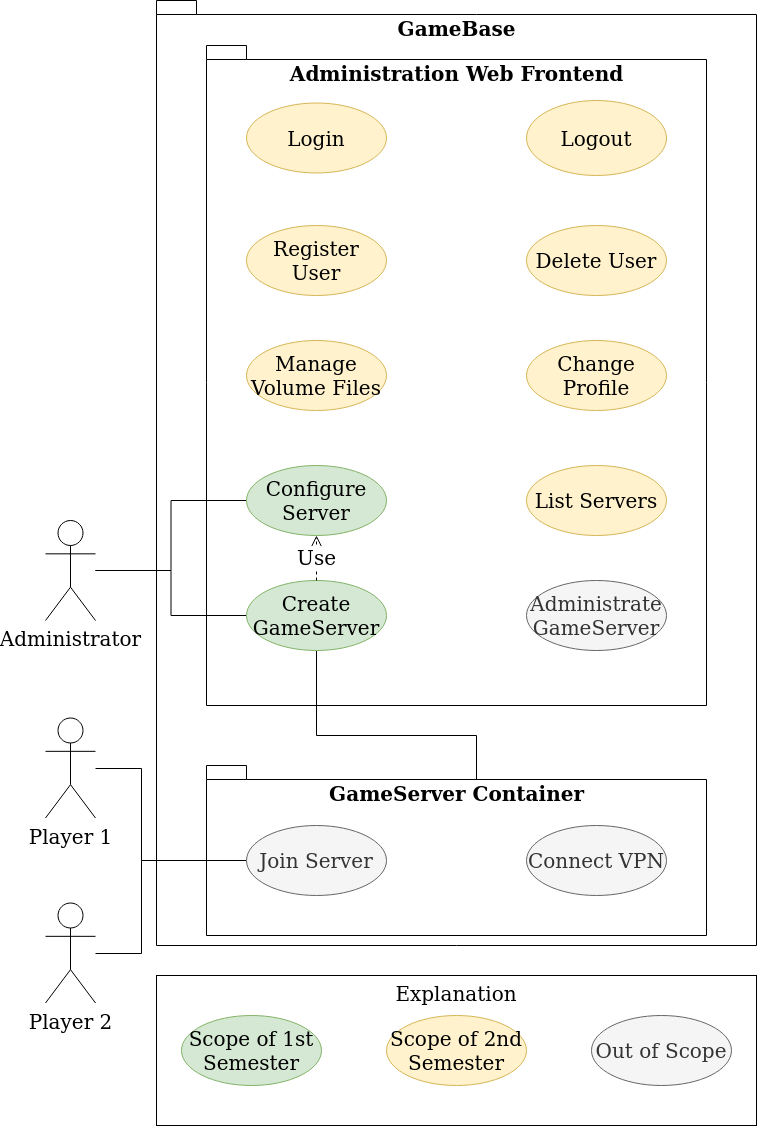
\includegraphics[width=\textwidth]{diagramms/Use_Case_Diagramm.png}
	\caption{Use Case Diagramm}
	\label{fig:ucd}
\end{figure}
Players are featured in our diagram even though they are not interacting with our application directly because after all connecting to the servers is a crucial part of our system.

Administration of the game servers with game specific features like \emph{kicking}, \emph{banning} and \emph{map rotation} is out of scope. This is due to the variety of games and their systems that handle these actions independently as we want to offer an experience of settings up any kind of game servers.

The main use case of our application is the easy management of game server containers created by Docker and having them deployed automatically to \gls{k8s}. We split up its functionality into two semester.

\chapter{Specific Requirements}
% [This section of the SRS should contain all the software requirements to a level of detail sufficient to enable designers to design a system to satisfy those requirements, and testers to test that the system satisfies those requirements.   When using use-case modeling, these requirements are captured in the Use-Cases and the applicable supplementary specifications.  If use-case modeling is not used, the outline for supplementary specifications may be inserted directly into this section, as shown below.]

\section{Functionality - Backend}
% [This section describes the functional requirements of the system for those requirements which are expressed in the natural language style. For many applications, this may constitute the bulk of the SRS Package and thought should be given to the organization of this section. This section is typically organized by feature, but alternative organization methods may also be appropriate, for example, organization by user or organization by subsystem.  Functional requirements may include feature sets, capabilities, and security.

% Where application development tools, such as requirements tools, modeling tools, etc., are employed to capture the functionality, this section document will refer to the availability of that data, indicating the location and name of the tool that is used to capture the data.]

The backend's task is to orchestrate Docker container. The orchestration method depends on the selected deployment. It can either be native or a 3rd party provider like \gls{k8s} or \gls{aws}. The user can choose a game server template on the frontend side, and the backend takes care of it being deployed as a container.

\subsection{Server Management and Creation (3rd semester)}
Through the frontend the user should be able to create any kind of game server containers and manage them. The template can either be:
\begin{itemize}
	\item an already pre-built one 
	\item or a custom made \gls{k8s} definition.
\end{itemize}
 
 
The functionality of management contains:
\begin{itemize}
	\item Start, stop and kill server
	\item Create container
	\item Configuring server (ports, player slots, RAM usage, ...)
%	\item Select deployment method
%	\item Recreating container (equals reinstallation)
\end{itemize}

\subsection{Status Reporting (4th semester)}
For better troubleshooting and further, concise information about a user's container, a status reporting system will be introduced. Example status can be:
\begin{itemize}
	\item Building...
	\item Starting...
	\item Running
	\item Stopping...
	\item Stopped
	\item Unknown
\end{itemize}

% \subsection{Volume Management (4th semester)}
% The client should be able to access server files inside a container via FTP/SFTP. This functionality can also include backup server files and make restoring accessible through the frontend.

\subsection{User System (3rd + 4th semester)}
At registration, the data provided by the user is stored in the \gls{k8s} cluster. It is needed to log in, edit the profile and also provides the basis for a permission system. According use cases are:

\begin{itemize}
	\item Register
	\item Log in
	\item Log out
	\item Change profile
	%\item Delete profile
\end{itemize}

As of defined use case scopes, in the 3rd semester, we firstly stick to only one account with Basic authentication. Later on, we implement a JWT Bearer authentication.

\subsection{Template Parsing ((3rd +) 4th semester)}
If the user chooses not to use a pre-built template, they can provide a custom made template as \gls{yaml}. After submitting their template, the backend parses it and feeds it with additional data that is required for \gls{k8s} deployment at the end. 

The backend is needed to separate the user interface from the actual interaction with the \gls{k8s} cluster. It manages user input before processing a user's adjusted request to the \gls{k8s} cluster.

% \subsection{<Functional Requirement One>}
% [The requirement description.]

\subsection{Read and Parse Data Passed by API Endpoints}
For the communication between both sides (frontend and backend) a universal data format is needed, therefore JSON is used. The frontend sends data in JSON to the backend in form of a request via an HTTP client and waits for a response from the backend which also answers with JSON.

It's important to validate input and output data in order to avoid malfunctions or possible abuse of undetected bugs. In order to provide a common \gls{dto} interface, we decide to use \textit{OpenAPI Specification}. It's used to define a REST interface in \gls{yaml} which the code generators for serversided and clientsided codes uses.

\subsection{Provide Data}
After data is requested from the frontend and the user is allowed to do so, the backend sends out the previously mentioned \gls{dto} objects. If an error occurs during requests, then an exception \gls{dto} will be returned instead. It contains
\begin{enumerate}
	\item ID of affected container
	\item Short code of exception
	\item Detailed description of exception
\end{enumerate} 

\section{Functionality - Frontend}
%[This section describes the functional requirements of the system for those requirements which are expressed in the natural language style. For many applications, this may constitute the bulk of the SRS Package and thought should be given to the organization of this section. This section is typically organized by feature, but alternative organization methods may also be appropriate, for example, organization by user or organization by subsystem.  Functional requirements may include feature sets, capabilities, and security.

% Where application development tools, such as requirements tools, modeling tools, etc., are employed to capture the functionality, this section document will refer to the availability of that data, indicating the location and name of the tool that is used to capture the data.]

The frontend provides an user interface for the users to interact with and is able to request data from the data backend. The following subsections explain the types of data the frontend can request. Each of the subsections corresponds to one or more use cases.

The user interface exposes several highly abstracted options for investigating and controlling containers to users through the app server system. Users should be able to deploy containers in very few steps (ideally a single click) which can be achieved by using same default configurations. According use cases are:

\begin{itemize}
    \item Request deployment
    \item Cancel deployment
    \item View deployment/container status
%    \item View reports/logs/metrics
\end{itemize}

You can see some use cases here:
\begin{itemize}
	\item \href{https://gamebase.pages.gitlab.tandashi.de/documentation/UCCreateGameServer.pdf}{Create Gameserver}
	\item \href{https://gamebase.pages.gitlab.tandashi.de/documentation/UCConfigureGameServer.pdf}{Configure Gameserver}
	% TODO
\end{itemize}

\section{Usability}
% [This section should include all of those requirements that affect usability. For example,
% \begin{itemize}
% 	\item specify the required training time for a normal users and a power user to become productive at particular operations
% 	\item specify measurable task times for typical tasks or base the new system’s usability requirements on other systems that the users know and like
% 	\item specify requirement to conform to common usability standards, such as IBM’s CUA standards Microsoft’s GUI standards]
% \end{itemize}
We will build the user interface intuitive, so that a new user does not necessarily need an explanation or in-depth training, even if our users don't know what containers are or how they work they should be able and comfortable with the deployment. For advanced users, when providing a custom \gls{k8s} template, they have to refer to \gls{k8s}'s documentation.


\section{Reliability}
% [Requirements for reliability of the system should be specified here. Some suggestions follow:
% \begin{itemize}
% 	\item Availability—specify the percentage of time available ( xx.xx%), hours of use, maintenance access, degraded mode operations, etc.
% 	\item Mean Time Between Failures (MTBF) — this is usually specified in hours, but it could also be specified in terms of days, months or years.
% 	\item Mean Time To Repair (MTTR)—how long is the system allowed to be out of operation after it has failed?
% 	\item Accuracy—specify precision (resolution) and accuracy (by some known standard) that is required in the system’s output.
% 	\item Maximum Bugs or Defect Rate—usually expressed in terms of bugs per thousand of lines of code (bugs/KLOC) or bugs per function-point( bugs/function-point).
% 	\item Bugs or Defect Rate—categorized in terms of minor, significant, and critical bugs: the requirement(s) must define what is meant by a “critical” bug; for example, complete loss of data or a complete inability to use certain parts of the system’s functionality.]
% \end{itemize}

% \subsection{<Reliability Requirement One>}
% [The requirement description.]

\subsection{Availability}
Our software won't be only used personally, but we also think about a commercial usage.
In case of personal usage, we cannot make any real assessment of availability. But we can have a passive effect on it e. g. by providing bug fixes as soon as possible.
On commercial usage, availability depends rather on the provider/hoster. Most of the time, most providers advertise with an update of 99.9\%.

\subsection{Mean Time Between Failures \& Mean Time To Repair}
If the application fails due an hardware issue, then the mean times are up to one's hosting provider. Since the ensured uptime of most hosting providers is 99.9\%, they try to fix the issue within a few minutes. However, if the application fails due a bug in our code, it is possible to revert to a previous version that has worked fine. This means we need to be careful about backward compatibility issues.

\subsection{Accuracy}
The status data which is displayed to users should be as close to realtime as possible. This is because the software has to interact with live systems and we want our users to be capable of making relevant decisions at all times. The fulfillment of this requirement is likely to depend on the individual hosting solution of our users and in this case outside of our control. Otherwise we should be able to ensure this by preferring both fast and efficient implementations and consequently, algorithms.

\subsection{Bug Classes}
We classify bugs which might appear in the software into either one of these two categories:

\begin{itemize}
    \item \textbf{Critical bug}: A critical bug occurs when the users are not able to use the application at all. A data breach or other condition where data that is supposed to be secret becomes publicly accessible is also considered a critical bug.
    \item \textbf{Non-critical bug}: A non-critical bug appears when the user can use the application but it appears glitched but the user experience is just slightly impacted. Crucially, bugs in this category have minimal impact on the use cases as outlined in this specification.
\end{itemize}

\section{Performance}
%[The system’s performance characteristics should be outlined in this section. Include specific response times. Where applicable, reference related Use Cases by name.
 %\begin{itemize}
 %	\item response time for a transaction (average, maximum)
 %	\item throughput, for example, transactions per second
 %	\item capacity, for example, the number of customers or transactions the system can accommodate
%	\item degradation modes (what is the acceptable mode of operation when the system has been degraded in some manner)
%	\item resource utilization, such as memory, disk, communications, etc.
 %\end{itemize}]
Performance is a significant aspect for fluent usage and operation.

\subsection{Response Time}
Our users' resources and requirements to our software may vary. This leads to different results which cannot be explicitly predicted or affected by us. A contribution to response can be made by following our guidelines during development and testing.

For instance, by using \emph{GoLang}, its parallelism algorithm should provide a better base of finishing concurrent task faster and safer.

\subsection{Throughput}
We don't expect a high volume of data transfer when using our software on personal purpose. If it comes to a bigger environment as in hosting and selling game servers, it's possible to scale our application as it is build with Docker. 


\subsection{Capacity}
By optimizing our Docker builds, we try to keep the size of volume layers as compact as possible. This guarantees faster deployment.


\subsection{Degradation Modes}
The application should under any circumstance maintain links or access to the container after for example the frontend has crashed. It should be able to recover by trying to restart itself. Otherwise the application should try to shutdown any running container associated with GameBase safely and gracefully. 

% \subsection{Resource utilization}

\section{Supportability}
% [This section indicates any requirements that will enhance the supportability or maintainability of the system being built, including coding standards, naming conventions, class libraries, maintenance access, maintenance utilities.]
Our frontend and backend will be clearly separated. A benefit is that each component acts independently and thus can be maintained separately without getting in conflicts with other components - unless a breaking change is planned, obviously. We try to stick to naming conventions which are common in the used technologies. We especially value practices which lead to the writing of clean code. By properly documenting code through comments and backing documents we make it easy to understand our infrastructure and increase maintainability.

\subsection{Coding Guidelines}
As we use different programming languages, different code styles which are common among these are present. We might try out some tools like \emph{CheckStyle} or internal formatter (JetBrains IDEs) to check code formatting and show warnings if a snippet is not compliant. \\

These are the code conventions we stick to:
\begin{itemize}
	\item \textbf{Go}: \href{https://golang.org/doc/effective_go.html}{Effective Go}
	\item \textbf{TypeScript}: \href{https://github.com/microsoft/TypeScript/wiki/Coding-guidelines}{Microsoft's TypeScript coding guidelines}
	\item \textbf{TypeScript/Angular}: \href{https://angular.io/guide/styleguide}{Angular Style Guide}
\end{itemize}

\subsection{Quality Assurance}
\label{sec:support_qa}
We want to develop quality software. As a measurement, unit/integration tests and a basic concept are quintessential. We integrate these steps in three levels:
\begin{itemize}
	\item \textbf{Upon concept}: Before starting developing, the person who just assigned themselves an issue needs to create a concept for solving the problem first. This doesn't have to be very explicitly detailed, but at least show the kind of tools or approaches you're trying to use to combat the problem. Afterwards, the concept is reviewed by another team member, ideally in form of peer reviews. If both agree to the changes to be made, the assignee can continue with development.
	\item \textbf{After development}: After a contributor has finished developing, a second reviews takes place. The reviewee should at least run the tests written by the contributor on either of their workstations and check the pipeline for positive outcomes. If both agree on what they have discussed, the changes are merged.
	\item \textbf{CI/CD}: During development process, we test bleeding edge code in CI bots. Those run unit and integration tests. Additionally, \emph{SonarQube} is used in order to detect common coding mistakes or code smells. The developer decides whether to fix them or not, but also has to make sure that a certain threshold for declining the build is not reached.
\end{itemize}

\section{Design Constraints}
% [This section should indicate any design constraints on the system being built. Design constraints represent design decisions that have been mandated and must be adhered to.  Examples include software languages, software process requirements, prescribed use of developmental tools, architectural and design constraints, purchased components, class libraries, etc.]

\subsection{Usage of Software Languages and Frameworks}
For the frontend we will use Angular and Nebular. Angular is one of popular frameworks that allows you to write modular websites in TypeScript. It updates content of a site dynamically which doesn't necessarily require refreshing the page. One can also develop single components and reuse them all over the application. An example component could be a login form, a profile card or dashboard widgets. Aside from that, if we need any kind of \gls{dto}s that have to be used in frontend but are dependent on backend, there are libraries available that enables converting simple \gls{dto}s into TypeScript classes. Besides of creating components, services can be created which handle e. g. REST requests or guards which can be used as an interceptor in Angular Routing.
Nebular takes care of themeing and adds some more miscellaneous modules to Angular, such as an auth module that takes care of session handling. This allows a simple implementation of user login, logout and registration on the frontend side. 
To deploy our frontend, Angular provides an extra build command for production use. However, it generated static files that have to be served by a web server. We use \textbf{nginx} to do that. It enables redirects if needed too. \\

% TODO: BACKEND -> Web server?? K8s???
The container server in the backend will use the Docker SDK which is available in \emph{Go}. \emph{Go} claims to make it easy to build simple, reliable, and efficient software. Its concurrency mechanisms make it easy to write programs that get the most out of multicore and networked machines, while its novel type system enables flexible and modular program construction. \\

For REST communication, we use \textit{OpenAPI Specification}. It's a \gls{yaml} file which specifies endpoints for RESTful web services and follows the \textit{OpenAPI Specification}. It establishes a shared layer of \gls{dto} without creating redudancy in frontend and backend code. After definition of a \gls{yaml} file
\begin{itemize}
	\item \textit{ng-openapi-gen} for Angular frontend
	\item \textit{OpenAPI Generator} for Go backend
\end{itemize}
for server and client code. 

\subsection{Development Tools and Libraries}
To make development efficient, we're using the following tools:

\subsection*{Organization}
\begin{itemize}
	\item \textbf{Git}: Version control system
	\item \textbf{GitLab}: Version control remote server
    \item \textbf{YouTrack}: Project planning tool with time tracking.
	\item \textbf{GitLab CI}: Continuous integration service	
\end{itemize}

\subsection*{Frontend}
\begin{itemize}
    \item \textbf{JetBrains WebStorm}: Angular frontend development
	\item \textbf{NPM}: Node.js package manager
	\item \textbf{Protractor}: Integration tests of website
	\item \textbf{Karma}: Unit testing
\end{itemize}

\subsection*{Backend}
\begin{itemize}
	\item \textbf{JetBrains GoLand}: GoLang backend development
	\item \textbf{\gls{k8s} official Go library}: Interaction with \gls{k8s} clusters
\end{itemize}

\subsection*{Code Quality}
\begin{itemize}
	\item \textbf{Editorconfig}: Appopriate formatting for compliance of coding guidelines. (\textit{Note}: Usage of formatter might not always apply.)
	\item \textbf{TSLint}: TypeScript linting for usual TS coding guidelines compliance.
	\item \textbf{SonarQube}: Code Quality check on both frontend and backend
\end{itemize}

\section{Online User Documentation and Help System Requirements}
\begin{itemize}
	\item \textbf{Swagger}: Automatic documentation creation for REST APIs
	\item \textbf{In code documentation}: Relevant information for developer.
\end{itemize}

\section{Purchased Components}
% [This section describes any purchased components to be used with the system, any applicable licensing or usage restrictions, and any associated compatibility and interoperability or interface standards.]
\gls{na}

\section{Interfaces}
% [This section defines the interfaces that must be supported by the application. It should contain adequate specificity, protocols, ports and logical addresses, etc. so that the software can be developed and verified against the interface requirements.]

\subsection{User Interfaces}
% [Describe the user interfaces that are to be implemented by the software.]
To ensure that the user can interact with our system, we need to implement (at least) these interface items:
\begin{itemize}
	\item Angular web frontend
	\item Creation and control of containers
	\item Container status reporting
	\item Creation of custom templates
	% \item Attachment to container console
	% \item Server files management
	% \item Deployment method selection
	\item User management system
	\item Update reminder
\end{itemize}

\subsection{Hardware Interfaces}
% [This section defines any hardware interfaces that are to be supported by the software, including logical structure, physical addresses, expected behavior, etc. ]
We cannot make precise interface requirements for our software. The reason for this is that we want to develop our software that functions as a distributed environment.
\begin{itemize}
	\item \textbf{OS}: Should be supported by any OS that fulfill \href{https://www.docker.com/}{requirements of using Docker}.
	\item \textbf{Orchestration systems/providers}: \gls{k8s}, \gls{aws}, \gls{gcs}
\end{itemize}

\subsection{Software Interfaces}
% [This section describes software interfaces to other components of the software system. These may be purchased components, components reused from another application or components being developed for subsystems outside of the scope of this SRS but with which this software application must interact.]
A huge requirement/major dependency is access to host system's or user's provider's \gls{k8s} cluster. This is solved by passing a \textit{kubeconfig} file to the backend's container as volume bind in Docker.

\subsection{Communication Interfaces}
% [Describe any communications interfaces to other systems or devices such as local area networks, remote serial devices, etc.]
This depends on the \textit{kubeconfig}. It requires efficient permission in its specified \gls{k8s} for e. g. accessing namespaces or allow appliance of \gls{yaml} files defined by \gls{k8s}.

\section{Licensing Requirements}
% [Defines any licensing enforcement requirements or other usage restriction requirements that are to be exhibited by the software.]
We will use the GNU Affero General Public License v3.0. The permissions are conditioned on making available complete source code of licensed works and modifications, which include larger works using a licensed work, under the same license. Copyright and license notices must be preserved. Contributors provide an express grant of patent rights. When a modified version is used to provide a service over a network, the complete source code of the modified version must be made available. \\
\gls{tbd}

\section{Legal, Copyright, and Other Notices}
% [This section describes any necessary legal disclaimers, warranties, copyright notices, patent notice, wordmark, trademark, or logo compliance issues for the software.]
GameBase is not responsible for any kind of damage that is done when using our software. 
\gls{tbd}

\section{Applicable Standards}
% [This section describes by reference any applicable standard and the specific sections of any such standards which apply to the system being described. For example, this could include legal, quality and regulatory standards, industry standards for usability, interoperability, internationalization, operating system compliance, etc.]
In terms of code standard, please read section \ref{sec:support_qa}. \\

\gls{tbd}

\chapter{Supporting Information}
% [The supporting information makes the SRS easier to use.  It includes:
% \begin{itemize}
% 	\item Table of contents
% 	\item  Index
% 	\item Appendices
% \end{itemize}
% These may include use-case storyboards or user-interface prototypes. When appendices are included, the SRS should explicitly state whether or not the appendices are to be considered part of the requirements.]
If you want to reach out to use, feel free to write us an e-mail:
\begin{itemize}
	\item \href{mailto:gahr.leonhard@student.dhbw-karlsruhe.de}{Leonhard Gahr}
	\item \href{mailto:gehrsitz.norman@student.dhbw-karlsruhe.de}{Norman Gehrsitz}
	\item \href{mailto:lukas.stefan@student.dhbw-karlsruhe.de}{Stefan Lukas}
	\item \href{mailto:reis.kevin@student.dhbw-karlsruhe.de}{Kevin Reis}
\end{itemize}

Otherwise, take a look at section \ref{tab:references-tabview} for other possibilities to reach us out.
\end{document}